\documentclass[8pt]{beamer}
%\usetheme{CambridgeUS}
%\usecolortheme{dove}
\setbeamertemplate{caption}[numbered]
\setbeamertemplate{footline}[frame number]
\setbeamerfont{caption}{size=\scriptsize}
\usepackage[gen]{eurosym}
\usepackage{float}
\usepackage{moresize}
\pdfmapfile{+sansmathaccent.map}

\usepackage{tikz}
\usepackage{pgfpages}
\setbeamertemplate{background canvas}{
    \tikz \draw (current page.north west) rectangle (current page.south east);
        }
\pgfpagesuselayout{2 on 1}[letterpaper,border shrink=5mm]
\beamertemplatenavigationsymbolsempty
\usepackage{caption}
%\setbeameroption{show notes} %un-comment to see the notes
\setbeamerfont{note page}{size=\ssmall}
\graphicspath{{../input/}}
\usepackage[outdir=./]{epstopdf}

\begin{document}

\DeclareGraphicsExtensions{.eps}

\title{2010 EU-Wide CEBS Stress Tests}
%\author{Chase Ross}
%\date{March 23, 2016}

%\beamersetaveragebackground{black}
%\begin{frame}
%\frametitle{}

%\end{frame}
%\beamersetaveragebackground{white}

%\frame{\titlepage}

%\frame{\frametitle{Table of contents}\tableofcontents}

\frame{\frametitle{2010 EU-Wide CEBS Stress Tests}

\textbf{Background:} interconnection between a weak banking sector and over-indebted governments

\begin{itemize}
\item Obvious to the market that the fate of banks and sovereigns were closely linked $\rightarrow$ protection on European banks and sovereigns moved in lockstep beginning in Q1 2010 (see figure below)
\item But there was little transparency in banks' exposures, so investors assumed the worst for all banks and raised funding costs for everybody
 \end{itemize}
 
 
\vspace*{\fill}
\begin{figure}[h]
\noindent
\makebox[\textwidth]{\includegraphics[scale=.7 ]{chart.pdf}}%

\end{figure}


The test aimed to assess ``banks' ability to absorb further credit and market shocks...and their dependence on public support measures''; but the real value was in the clarity and transparency provided by the test (not unlike the 2009 SCAP)
}

\frame{\frametitle{}

\textbf{Test Design in a Nutshell}

\vspace{2mm}
Hurdle rate: 6\% Tier 1 Capital
\vspace*{\fill}
\begin{figure}[h]
\noindent
\makebox[\textwidth]{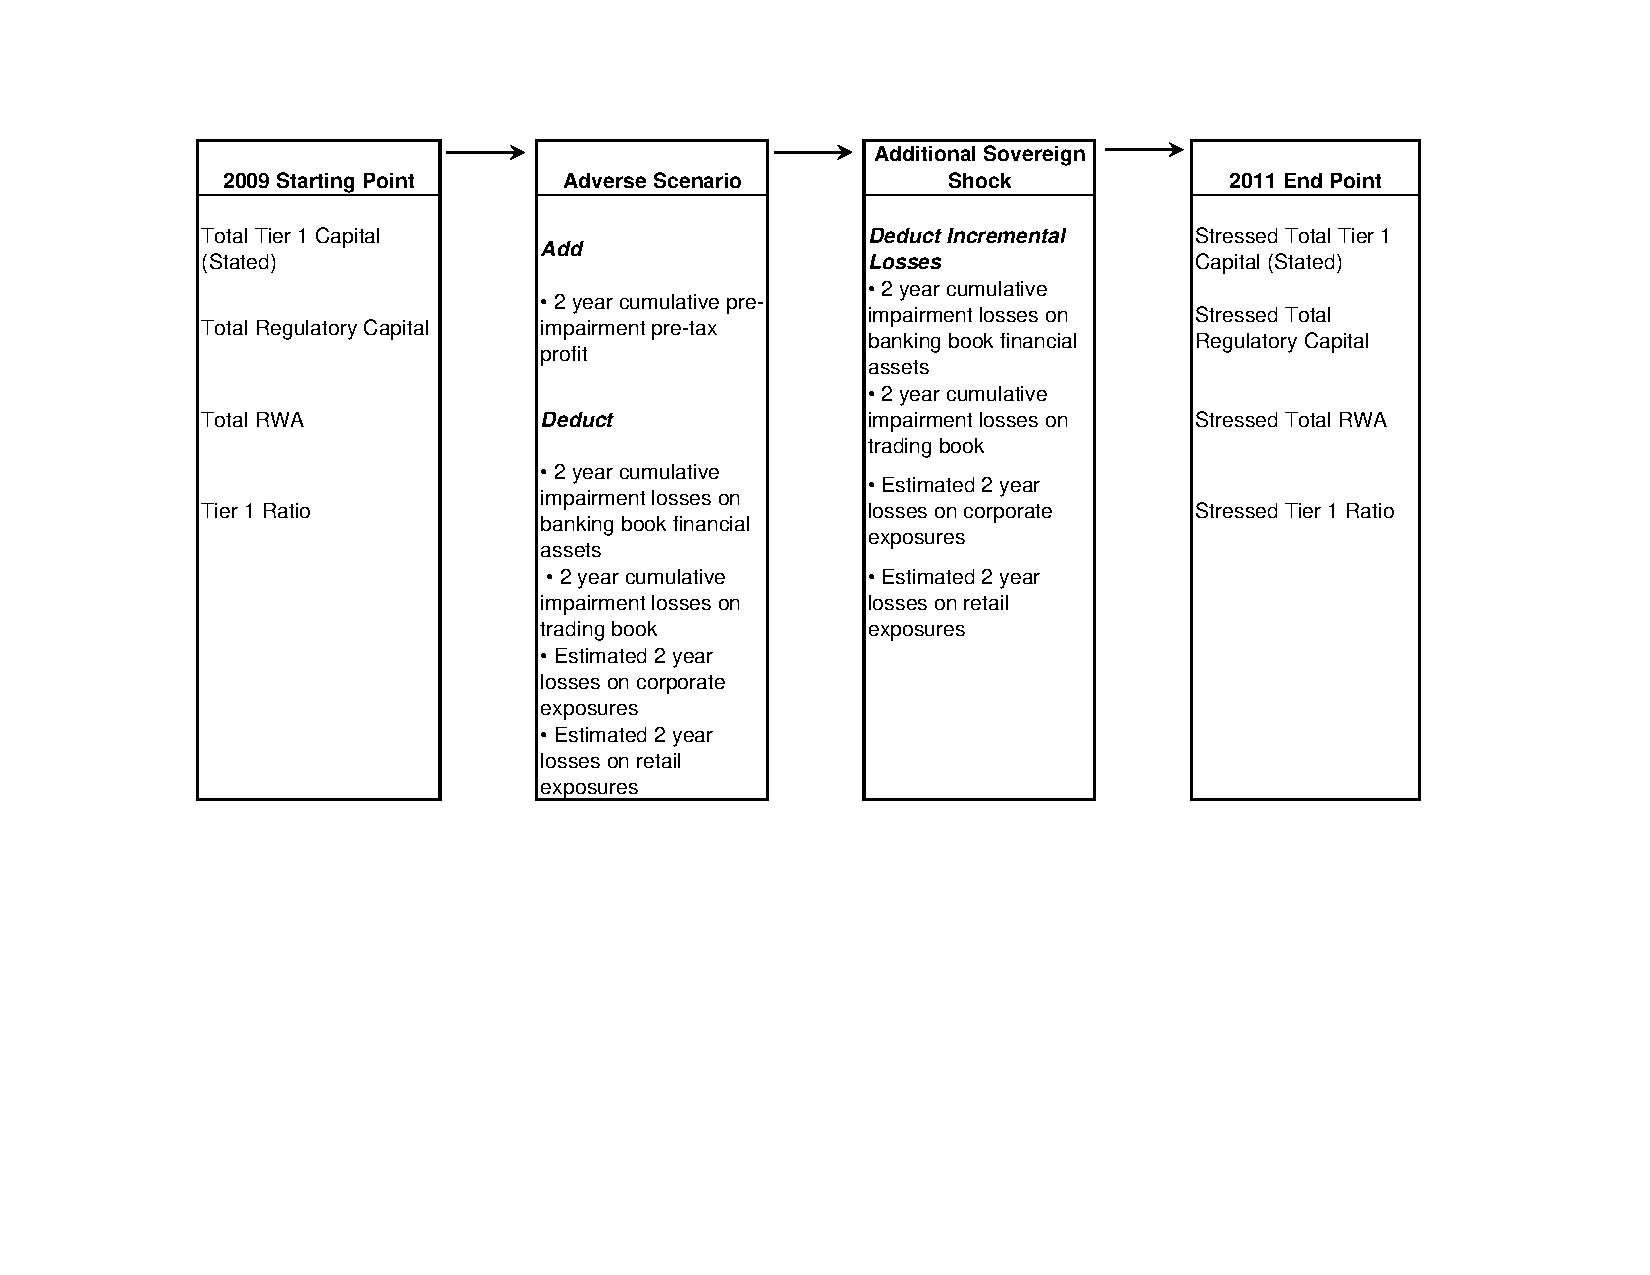
\includegraphics[scale=.52 ]{flowchart.pdf}}%

\end{figure}
}

\frame{\frametitle{ }
\begin{columns}[T] % align columns
\begin{column}{.48\textwidth}

\textbf{Results}

\begin{itemize}
\item Released July 2010.
\item Total capital needs of all failed banks: \euro{3.5} billion.
\item 7 banks failed; 2 of which already nationalized (only 1 Greek bank failed).
\item Interbank funding didn't ease; cost of protection remained  high.
\item SCAP-like: results were published in great detail (and the methodology was more transparent that SCAP).
\item Included sovereign support announced before July 2010.
\item 20 banks benefited from asset guarantees.
\item 34 benefited from \euro{170} bn of aggregate public capital, about 14\% of aggregate Tier 1 capital (ultimately increasing stressed Tier 1 capital by 1.2\%).
\end{itemize}


\end{column}%
\hfill%
\begin{column}{.48\textwidth}

\textbf{Key Design Decisions \& Credibility}

\vspace{2mm}

\begin{enumerate}
\item Inclusion of sovereign support.
\item Sovereign debt haircuts were applied to trading books but not banking books.
\item Forecast assumptions provided by national supervisors varied dramatically: for example, commercial real estate  prices were modeled to decline 55\% in Spain compared to 7\% in Greece.
%\item Optimistic pre-provision revenue forecasts. %(some banks forecast more PPNR in 2010 under the adverse scenario than actual numbers in 2009, probably due to extrapolating from high Q1 run rates)
\item CEBS, 27 national supervisors, the EU Commission, and the ECB worked together on the test.
\item Supervisors published the methodology of the stress test and its results at a very detailed level.
\item Low hurdle rate -- many expected 6\% core Tier 1.
\end{enumerate}


\end{column}%
\end{columns}
}


\end{document}
